% !TEX program  = xelatex
\documentclass[a4paper]{article}
\usepackage{amsmath}
\usepackage{amssymb}
\usepackage{enumerate}
\usepackage{amstext}
\usepackage{ctex}
%\usepackage{braket}
\usepackage[european]{circuitikz}
\usepackage{multirow}
\usepackage{graphicx}
\usepackage{subfig}
\usepackage{float}
\usepackage{url}
%\usepackage[table,xcdraw]{xcolor}
\usepackage{colortbl}
\usepackage{siunitx}
\usepackage{geometry}
\geometry{left=2.5cm,right=2.5cm,bottom=2.5cm,top=2.5cm}

\title{
%模电实验报告XI:有源RC滤波电路
}
%\author{匡院\quad 王石嵘\\161240065}
%\date{2019年5月23日}
\begin{document}
	\maketitle

\begin{figure}[H]
	\centering
	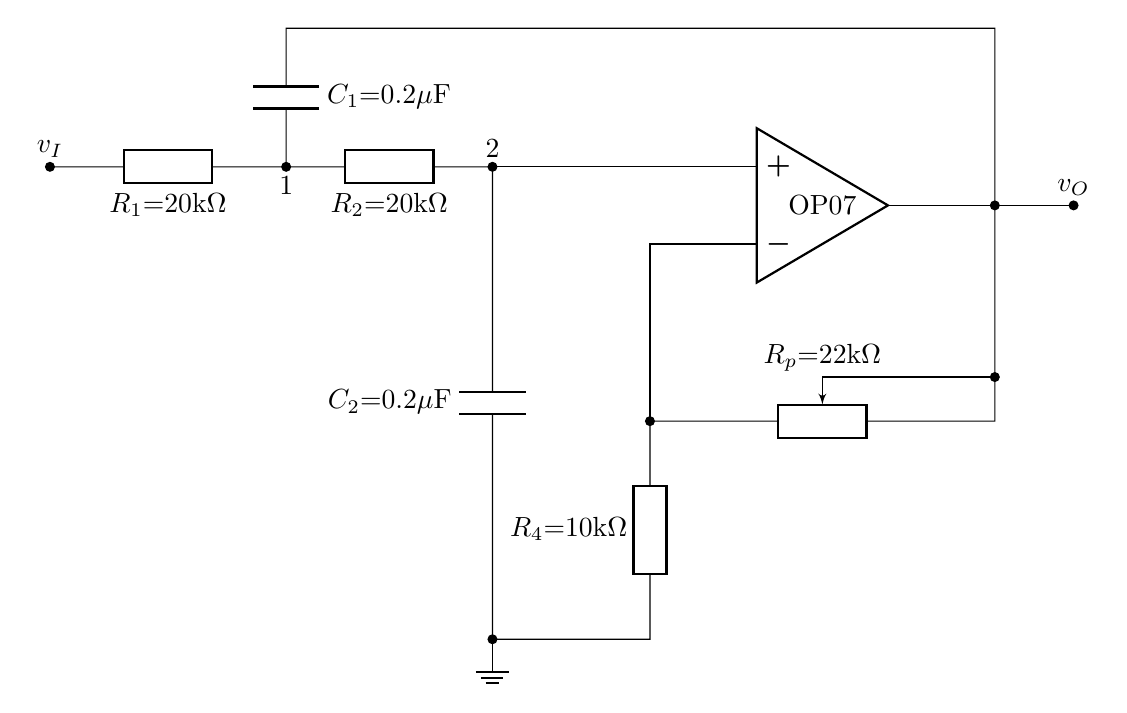
\begin{tikzpicture}[x = 2cm, y = 1.5cm]
	\draw (0,0) node[op amp, yscale = -1](AMP){} node{OP07};
	\draw (AMP.+) -- ++(-1.5,0) node[circ](N1){} node[anchor = south]{2}
	(AMP.-) -| ++(-0.5,-1.5) node[circ](N2){}
	(AMP.out) -- ++(0.5,0) node[circ](N3){};
	
	\draw let \p1 = (N1), \p2 = (N2), \p3 = (N3) in
	(N2) to [pR, l=$R_p{=}22\text{k}\Omega$, n=PR] ($(\x3,\y2)$) -- (N3) |- ++(-4.5,1.5) to [C, l=$C_1{=}0.2\mu\text{F}$] ($(\x3,\y1)+(-4.5,0)$) node[circ](N4){} node[anchor = north]{1} to [R, l_=$R_2{=}20\text{k}\Omega$] (N1) to [C, l_=$C_2{=}0.2\mu\text{F}$] ++(0,-4) node[circ]{} node[ground]{} -- ++(1,0) to [R, l=$R_4{=}10\text{k}\Omega$] (N2)
	;
	
	\draw (N3) -- ++(0.5,0) node[circ]{} node[anchor = south]{$v_O$};
	\draw (N4) to [R, l=$R_1{=}20\text{k}\Omega$] ++(-1.5,0) node[circ]{} node[anchor = south]{$v_I$};
	\draw let \p1 = (N1), \p2 = (N2), \p3 = (N3) in (PR.wiper) -- ++($(-\x2/2,0)+(\x3/2,0)$) node[circ]{};
	\end{tikzpicture}
	\caption{有限正增益低通二阶基本节电路图}\label{fig1}
\end{figure}

\end{document}